\documentclass{article}
\usepackage{tikz}
\usepackage{amsmath}

\begin{document}

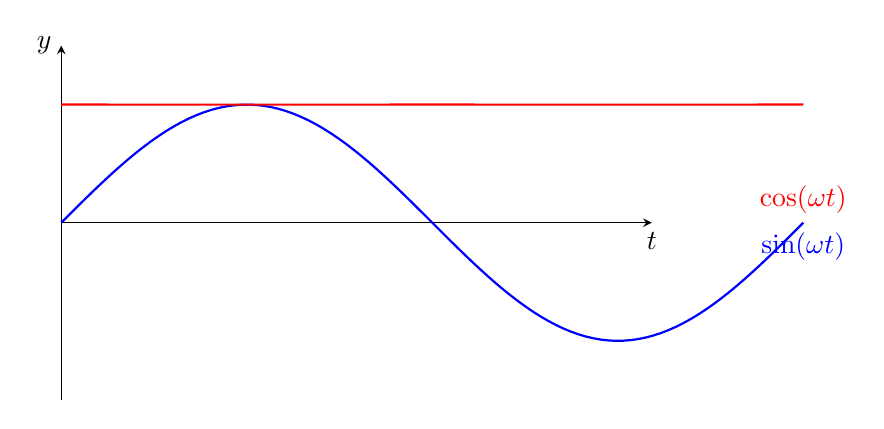
\begin{tikzpicture}[scale=1.5]
  % Axe des x
  \draw[-stealth] (0,0) -- (5,0) node[below] {$t$};
  % Axe des y
  \draw[-stealth] (0,-1.5) -- (0,1.5) node[left] {$y$};

  % Signal 1 (sinus)
  \draw[blue, thick, domain=0:2*pi, samples=100] plot ({\x}, {sin(\x r)});
  \node[blue, below] at (2*pi,0) {$\sin(\omega t)$};

  % Signal 2 (cosinus déphasé de 90 degrés)
  \draw[red, thick, domain=0:2*pi, samples=100] plot ({\x}, {cos(sin(\x r))});
  \node[red, above] at (2*pi,0) {$\cos(\omega t)$};
\end{tikzpicture}

\end{document}
